%%%%%%%%%%%%%%%%%%%%%%%%%%% Paper.tex %%%%%%%%%%%%%%%%%%%%%%%%%%%%%%%
% Template for producing ASME-format journal articles using LaTeX    %
% Written by   Harry H. Cheng, Professor and Director                %
%              Integration Engineering Laboratory                    %
%              Department of Mechanical and Aeronautical Engineering %
%              University of California                              %
%              Davis, CA 95616                                       %
%              Tel: (530) 752-5020 (office)                          %
%                   (530) 752-1028 (lab)                             %
%              Fax: (530) 752-4158                                   %
%              Email: hhcheng@ucdavis.edu                            %
%              WWW:   http://iel.ucdavis.edu/people/cheng.html       %
%              May 7, 1994                                           %
% Modified: February 16, 2001 by Harry H. Cheng                      %
% Modified: January  01, 2003 by Geoffrey R. Shiflett                %
% Use at your own risk, send complaints to /dev/null                 %
%%%%%%%%%%%%%%%%%%%%%%%%%%%%%%%%%%%%%%%%%%%%%%%%%%%%%%%%%%%%%%%%%%%%%%

%%% use twocolumn and 10pt options with the asme2e format
\documentclass[twocolumn,10pt]{asme2e}

\newcommand*{\captionsource}[2]{%
  \caption[{#1}]{%
    #1%
    \\\hspace{\linewidth}%
    \textbf{Source:} #2%
  }%
}

\usepackage{textcomp}
\usepackage[USenglish]{babel}    % English
\usepackage[ansinew]{inputenc}   % Output glyphs like 'ö' at all
%\usepackage[T1]{fontenc}         % Output glyphs like 'ö' in a nice font
\usepackage{graphicx}            % For loading graphic files
%\usepackage{a4wide}              % Smaller margins = more text per page.
\usepackage{fancyhdr}            % Fancy headings
\usepackage{longtable}           % For tables, that exceed one page
\usepackage{xspace}              % Geeft spaties na commando's die dat behoeven
%\usepackage{titling}
 

\usepackage{mathtools}             % Math packages
\let\proof\relax 
\let\endproof\relax
\usepackage{amsthm}
\usepackage{amsfonts}

%% The class has several options
%  onecolumn/twocolumn - format for one or two columns per page
%  10pt/11pt/12pt - use 10, 11, or 12 point font
%  oneside/twoside - format for oneside/twosided printing
%  final/draft - format for final/draft copy
%  cleanfoot - take out copyright info in footer leave page number
%  cleanhead - take out the conference banner on the title page
%  titlepage/notitlepage - put in titlepage or leave out titlepage
%  
%% The default is oneside, onecolumn, 10pt, final


\title{Determining Tire characteristics through data driven modeling}

%%% first author
\author{Eugene Figueiras
    \affiliation{
	BSC student\\
	TU Delft\\
    SN:0000000 
    }	
}

%%% second author
%%% remove the following entry for single author papers
%%% add more entries for additional authors
\author{Maarten Kleijwegt
    \affiliation{
	BSC student\\
	TU Delft\\
    SN:4113810 
    }	
}

%%% third author
%%% remove the following entry for single author papers
%%% add more entries for additional authors
\author{Nol R{\"o}mer
    \affiliation{
	BSC student\\
	TU Delft\\
    SN: 4391888
    }	
}

\author{Akash Soerdjbalie
    \affiliation{
	BSC student\\
	TU Delft\\
    SN: 4227174
    }	
}

\author{dr.ir. Tam{\'a}s Keviczky
    \affiliation{
	Associate Professor \\
	Delf Center for Systems and Control 
    }	
}
\author{Wil van Geest
    \affiliation{
	???\\
	Delft Center for Systems and Control\\
    }	
}
\begin{document}

\maketitle    

\begin{abstract}
Lorem ipsum dolor sit amet, consectetuer adipiscing elit. Maecenas porttitor congue massa. Fusce posuere, magna sed pulvinar ultricies, purus lectus malesuada libero, sit amet commodo magna eros quis urna.
Nunc viverra imperdiet enim. Fusce est. Vivamus a tellus.
Pellentesque habitant morbi tristique senectus et netus et malesuada fames ac turpis egestas. Proin pharetra nonummy pede. Mauris et orci.
\end{abstract}
\section{Introduction}
If you talk to racing enthusiasts you quickly find out one of the key components in any competition car are the tires. They provide the interface between all the components a race car consists of and the track it\textquotesingle s driving on. Therefore, tires dictate any behaviour a car is capable of. Those 4 foot sized patches of rubber make the difference between being able to make those quick sharp corners and spinning out of the ring. In daily traffic making those tires stick to the road can sometimes make the difference between life and death. In the United States alone, the National Highway Traffic Safety Administration (NHTSA) reports that 5 million crashes occurred in 2009 [59], causing over 30,000 deaths and 2 million injuries. 

Until now, driver safety systems in modern-cars have focussed on keeping the car in the linear regime while driving. For example, ABS prevents the wheels from slipping and traction control prevents the car from \textquotesingle breaking out\textquotesingle  of its path. However, when we look towards professional rally drivers we see that operating in the linear regime isn\textquotesingle t specifically necessary for driving safe. If we would be able to give the skills of a rally driver to driver assistance systems, or in the future autonomous cars, more accidents might be prevented. It would give forementioned systems more capabilities and options. Which might result in better accident prevention solutions.

This paper focuses on establishing a measurement setup and determining the tire characteristics of a small-scale RC car with it. It is a step towards achieving a good Nonlinear Model Predictive Control (NMPC) system. NMPC is a new control method which uses a dynamical model that can predict the motion of the car. Therefore, this system is able to let the car make evasive maneuvers up to the nonlinear regime of driving. In order to obtain a good dynamical model for the NMPC, tire characteristics are required. There are a few ways to obtain these characteristics. Normally, these characteristics are determined using special test rigs where only the wheels are placed in. However, these characteristics are only valid for that given tire, in only that given condition( think of temperature, wornness and wetness of the tire) on only a single given surface. A lot of testing can be done to determine the characteristics of all tires in all conditions. Yet it would be far better if a car would be able to determine it\textquotesingle s characteristics using on board sensors such as GPS and Inertial Measurment Units or IMU\textquotesingle s. Testing with real cars and on-board sensors in a special test environment is a possibility. But developing and refining this technique on small scale RC cars first requires less resources such as large test tracks and expensive cars and tires. Let alone other expenses like experienced mechanics and drivers.Therefore, using a small-scale RC car equipped with sensors is by far the least expensive way to obtain these tire characteristics. These methods can then be scaled for actual cars.

This all concludes to the aim of this paper, which is determining the tire characteristics of a small scale RC car using only on board sensors. At first, some scientific background is given on the subject. After that, the experimental setup and data processing will be explained. Next, results will be discussed. Finally, the conclusion will be given. The paper also leaves some room for recommendations and acknowledgements.  


\section{Modelling}
In order to achieve Model Predictive Control, it\textquotesingle s important to build a valid model of the dynamics of the RC car. In order to do so, it\textquotesingle  s important to understand the tire characteristics of this vehicle. This means there has to be a model for the tire characteristics as well. To build such a model, Data-Driven Model Design is used. 
To analyse the data of the test rig, a dynamical model is necessary. Accuracy of a dynamical model is closely related to the complexity of the model. However, due to the computational burden of these systems, a relative simple yet accurate model is necessary. Therefore, the Bicycle Model is chosen (Bron: 2014-01-0841 google drive pdf FIXME). With this model, it is possible to generate real time data that is still accurate. 

\begin{figure}
	\centering
		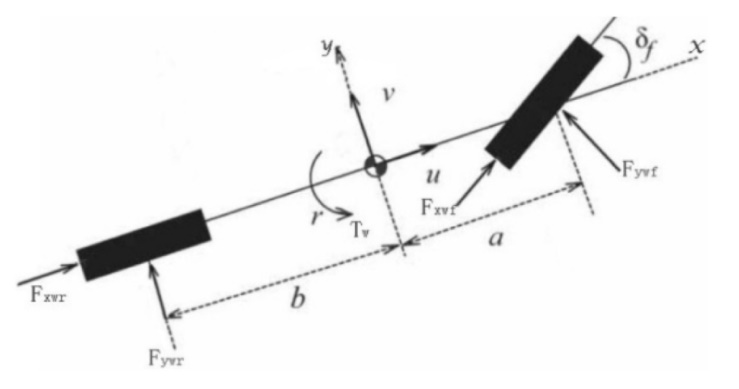
\includegraphics[scale=0.5]{figure/bicyclemodel.jpg}
	\label{fig:bicyclemodel}
	\caption{Bicycle model}
\end{figure}
Another suitable tire model would be the Dugoff tire model. This model provides a less accurate representation of the tire characteristics, but requires less variables. Even though fewer variables are needed though, more of the variables are unknown. Therefore, the Magic Formula model is easier to apply and gives a more accurate result, so to simplify calculations without a reduced quality of the final results, the Magic Formula model is chosen. 

\subsection{The Bicycle Model}
In the Bicycle Model, the car is represented as a rigid, two-dimensional, two-wheel vehicle with a xyz-coordinate system is fixed to the car frame. The front wheels are represented as one wheel and so are the rear wheels, as visible in figure \ref{fig:bicyclemodel}. This model comes with some important assumptions so there are some restrictions to test settings as well. The car should not move in the vertical (z-) position, nor rotate in the roll and pitch directions (around the x- and y- axes respectively). Therefore, movements are only possible in the x- and y-direction and as a rotation around the z-axis(yaw). 
	Furthermore, the bicycle model is divided in two parts: the linear and the nonlinear bicycle model. In general, a linear model is used for simplicity of the controller. Even though the performance of this model degrades at the limits of friction, it is demonstrated that using a linear tire model is still a good way of modelling (BRON: 2012-thesis-Kritayakirana GOOGLE DRIVE page 9). Even though, the non-linear bicycle model gives an even more accurate approximation of vehicle dynamics, and is therefore used.
	In the linear bicycle model, constant longitudinal velocity is assumed and lateral acceleration should not exceed 0.3 g . In order to meet these assumptions, the vehicle is not allowed to accelerate in the longitudinal direction while cornering. Therefore, data is not valid in the first seconds of each cornering test where the car has to accelerate. For the longitudinal motion tests however, it is necessary to accelerate and decelerate on the straight. If we still want to use the linear Bicycle Model for these experiments, the accelerations and decelerations cannot be very high. Otherwise this will result in inaccurate values given by this model.
	However, in some cases it will be helpful to use the nonlinear Bicycle Model. The limitations stated in the previous section will not occur. The nonlinear Bicycle Model will be used for tests where the longitudinal and lateral accelerations are high. This model comes with a larger set of equations and variables, and is solvable if the distribution of forces on the front and rear tires is known. In order to solve the equations, we assume a 50-50 distribution on these wheels, which makes sense if both the front and rear wheels are spinning at the same time. Because the wheels are connected to the same motor ,through differentials, and share the same properties, the forces acting on the wheels are approximately the same. 
	
\subsection{The Magic Formula}	
When the forces acting on the wheels of the car are known, thanks to the bicycle model values can be found to determine the slip angle \(\alpha\) and the slip ratio \(\kappa\). With these known, the tire characteristics can be determined using the Magic Formula tire model
 \ref{eq:magicformulaA}. 
\begin{equation}
	[F_{xwi} ,F_{ywi}] = MF(F_{zi},\alpha_{i},\kappa_{i},\mu) (i = f,r)
	\label{eq:magicformulaA} 
\end{equation}

In equation 1, the longitudinal force F_{x} and the lateral force F_{y} are calculated, using a the magic formula (MF) that depends on the gravitational force F_{z}, the slip angle \(\alpha\), the slip ratio \(\kappa\) and the friction coefficient \(\mu\). Except \(\mu\), all these variables are defined for two points on the bicycle model: the front wheel (f) and the rear wheel (r). 
	Equation \ref{eq:magicformulaA} can also be written as equation \ref{eq:magicformulaB}, which is stated by R.T. Uil of Eindhoven University. In this equation, variables B, C, D and E are introduced. B stands for the stiffness factor, C stands for the shape factor, D stands for the peak value and E stands for the curvature factor. This basic representation of the magic formula forms a graph that approximates the measured data and forms the tire characteristics of the vehicle. 

 \ref{eq:magicformulaB}. 
\begin{equation}
	R(\(\kappa\)) = D*sin{C*arctan[B*(1-E)*\(\kappa\)+E*arctan(B*\(\kappa\))]}
	\label{eq:magicformulaB} 
\end{equation}

\section{Experimental setup}
 

In order to determine the tire characteristics of the scaled vehicle, a good testbed is necessary. In this section the experimental setup used to gather the data needed for determining the tire characteristic is discussed.\\
The experimental setup consists of a modified scaled RC car with an on board IMU, and a tachometer on each wheel. Moreover, a motion capture system or MoCap was used to provide millimeter precision locating. A note should be made here that the testbed was recycled from earlier research into the same subject made by [reference to last group's paper]. As stated in their paper there were a lot of software related problems with the car. Therefore the limited time we had for this research, was mostly used for programming the test setup and creating a working system. We therefore choose to ignore any physical design faults, at least in the beginning, to fix these problems first. This made our results susceptible to these faults in the end. Later work might improve on this. 

Usually a MoCap system can't be regarded as an \textquotesingle on-board sensor\textquotesingle ,seeing as it requires an external area with set up with camera's. However in our case it was used as a replacement for a gps sensor. A gps sensor would be less desirable in our situation as the accuracy doesn't scale down with the car. Moreover a MoCap system enables us to do testing inside. Something which is troubling at best when tried with a GPS system. Moreover, most of the MoCap system was delivered as is. Which meant all of the data would be presented in ROS. And the sampling rate of the mocap would be set in stone at 120HZ.

The scaled RC car is a Losi TEN Rally-X. It is a 1:10 scale car with 4WD.  
Each wheel was fitted with it\textquotesingle s own hall effect sensor which generates a pulse every time one of the magnets inside the rim passes it. Many of the first tests were done using only 2 magnets giving only 1 pulse per \(pi\) radial turned. However after most of the testing was done we figured out a rim with 24 magnets would be much more suited. To fit both the 2 magnets and the 24 magnet versions to the car a set of custom 3d printed rims were created. Using the 24 magnet version a pulse every \(pi/12\) radial was generated giving a higher resolution. Finally, the car\textquotesingle s suspension is replaced with stiff turnbuckle rods to eliminate the degrees of freedom of roll and pitch, to meet the assumptions of the Bicycle model.

\begin{figure}
  \centering
    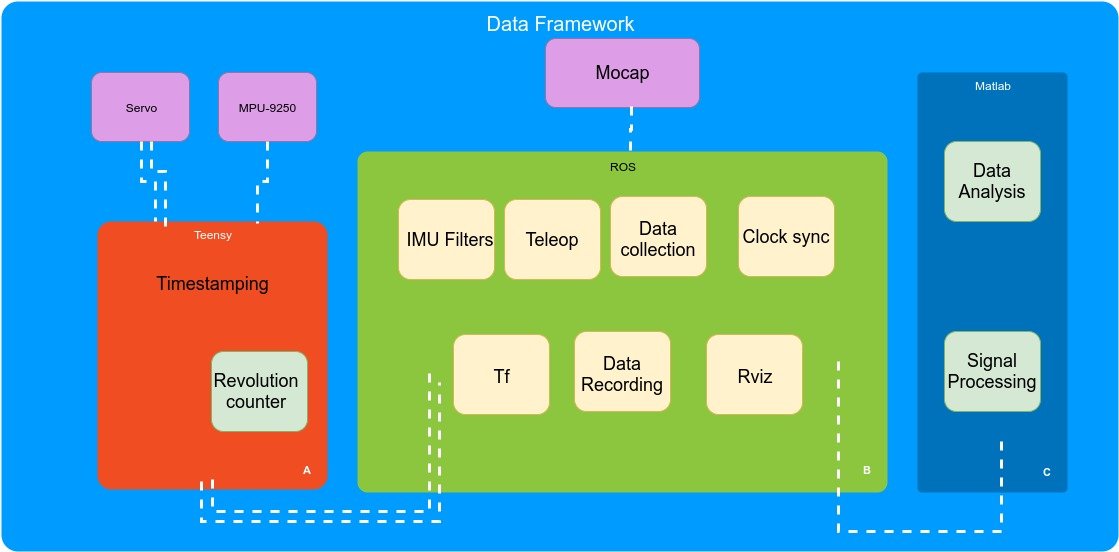
\includegraphics[scale=0.22]{figure/DataFramework.jpg}
  \caption{Data acquisition framework}
  \label{fig:DonutFramework} 
\end{figure}

Data acquisition was done using a ROS (Robot Operating System) based system. The sensors were read using a Teensy 3.6 protyping board running a costum ROSserial node, connected to a Raspberry pi 3b running ROS. The MoCap connected to the system utilizig the labs Wi-Fi network. Further communication was done using a self written ROS package. After data collection further processing was done using Matlab.Figure
\ref{fig:DonutFramework} further eleborates the Data acquisition framework.

ROS was chosen as basis for the system for 3 reasons. First, there was already a lot of experience in the research team using ROS which made it an easy choice to use to fix a lot of the problems with the testbed. Second the MoCap generated it's data already in ROS. Which meant combining everything in ROS would be a simplification. Last ROS offers really easy Data recording options called ROSbags. These can be easily imported in to MATLAB to do further analysis.

Seeing as the MoCap already delivered her data at a sampling rate of 120hz. It was easy to pick this as the target sampling rate for the whole system. Seeing as our speeds reach somewhere in between 0-20[m/s] this would mean a maximum of 0.167[m] traveled per sample. This felt accurate enough for our purpose.

The experiments that we conducted can be classified into three groups. The first set of experiments are the ones on the straight (longitudinal motion). During these we accelerated and braked while driving straight ahead. The second set are the steady state cornering experiments (lateral motion). Steady state cornering means cornering at a constant longitudinal velocity and constant steering angle. The first group of experiments focuses on longitudinal forces and slip ratios, while the second group focuses on lateral forces and slip angles. The tests were separated in order to distinguish longitudinal and lateral motion (Recommendation Barys Shyrokau). Finally, the third set of experiments are of combined motion. These tests take both lateral and longitudinal motion into account. 
	Variables of the tests are acceleration/deceleration for longitudinal motion, longitudinal velocity and steering angle for lateral motion, and these three combined for  combined motion. The variables were slightly increased each experiment in order to determine the \textquotesingle borderline\textquotesingle  between linear and nonlinear behaviour is.
	
The experimental data is collected in rosbags and processed afterwards. This makes it possible to filter the noise from the IMU with a Zero-Phase Low Pass Butterworth Filter. This is a non-causal filter with a phase slope of zero. This eliminates any delay, commonly caused by causal filters. The Low Pass filter is of the 20th order, in order to approach an ideal \textquotesingle Brick wall Response\textquotesingle .
	\begin{figure}
	\centering
	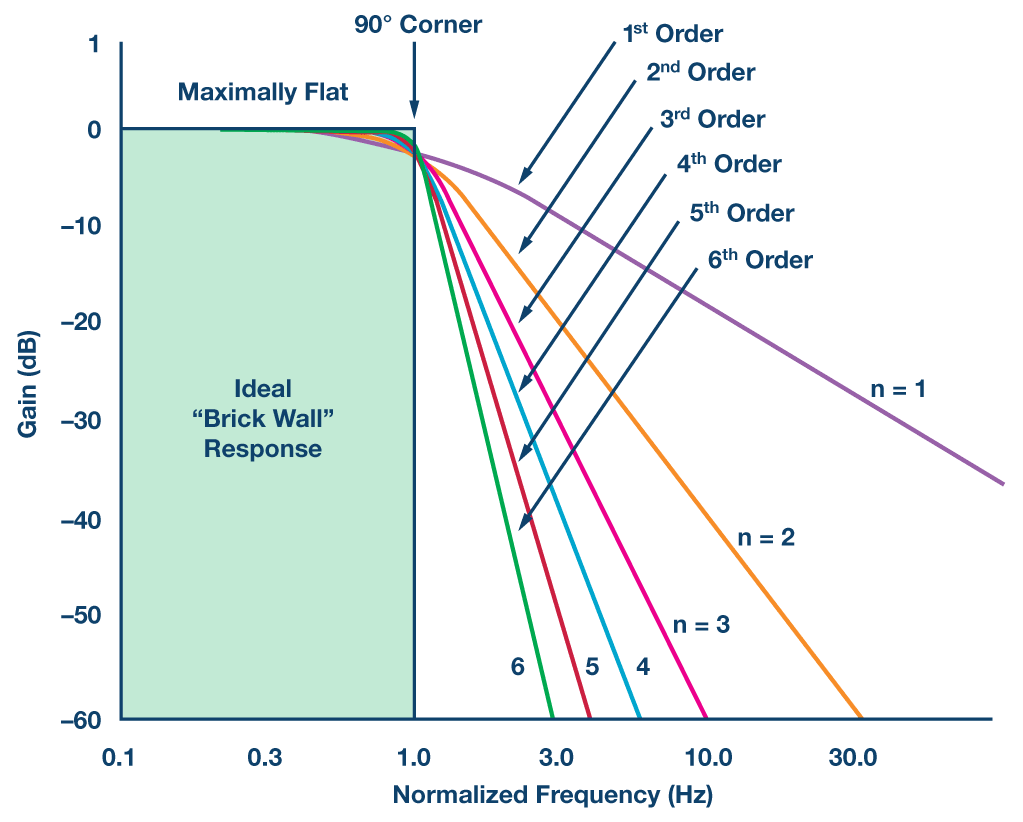
\includegraphics[scale=0.17]{figure/brickwall.png}
	\caption{Brick wall response}
	%\captionsource{Caption}{(http://www.electronics-tutorials.ws/filter/filter_8.html)}
	\label{fig:brickwall}
	\end{figure}


 
\subsection{Longitudinal slip}
Differentiating the Mocap Data creates a lot of noise. Integrating the IMU data results in a much more stable velocity signal. This signal combined with the data from the Hall Effect Sensors is used to calculate the Longitudinal slip ratio using the following formulas:
\begin{figure}
	\centering
	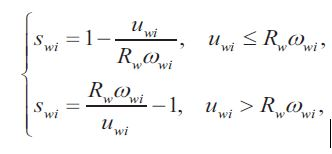
\includegraphics[scale=0.4]{figure/Longitudonalslip}
	\caption{Longitudinal slip}
	\label{fig:brickwall}
	\end{figure}

\subsection{Forces}
The forces, acting along the y-axis of the body fixed frame of the car, are calculated using the equations of motion. As mentioned earlier there are three types of experiments that were conducted. This makes it easier to obtain these forces.

\begin{figure}
	\centering
	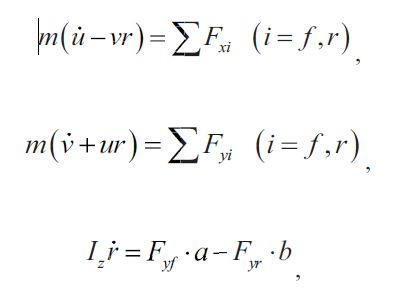
\includegraphics[scale=0.4]{figure/Equationsofmotion}
	\caption{equations of motion}
	\label{fig:brickwall}
	\end{figure}

Where the forces on the wheels are obtained by formula \ref{eq:magicformula}

\subsection{Curve Fitting}
After obtaining the forces, slip ratio and slip angles, from multiple bags, the data is curve fitted in order to obtain the 4 parameters from the magic formula.
 


\section{Discussion}
\section{Conclusion}
%%%%%%%%%%%%%%%%%%%%%%%%%%%%%%%%%%%%%%%%%%%%%%%%%%%%%%%%%%%%%%%%%%%%%%






\end{document}